\documentclass{beamer}
\usepackage[latin1]{inputenc}
\usepackage[T1]{fontenc}
\def\spanishoptions{chile}
\usepackage[spanish]{babel}
\selectlanguage{spanish}
\usepackage{amssymb}
\usepackage{soul}
\usepackage{listings}
\usepackage{alltt}
\usepackage{underscore}
\usepackage{verbatim}
\usepackage{graphicx}
\usepackage{ae}
\usepackage{amsmath}
\usepackage{amsfonts}
\PassOptionsToPackage{pdflatex}{graphicx}
\usepackage{algorithm}
\usepackage{algorithmic}
\graphicspath{ {data/} }

\definecolor{listinggray}{gray}{0.9}
\definecolor{lbcolor}{rgb}{0.9,0.9,0.9}


\usefonttheme{professionalfonts}


\title[Dise�o y an�lisis de algoritmos]{Dise�o y an�lisis de algoritmos}
\subtitle{Comparaci�n de rendimiento entre algoritmos de selecci�n de medianas} 
\author[E. Regla]{Erik Regla} 
\institute[UTalca]{Universidad de Talca}
\date{\today} 

\begin{document}

\begin{frame}
  \titlepage
\end{frame}

\section{Descripci�n de las pruebas experimentales}

\begin{frame}
  Descripci�n de las pruebas
  \begin{itemize}
  	\item Tama�o: 11GB
  	\item $5\%$ de los elementos est�n repetidos
  	\item Distribuci�n uniforme
  	\item Se realizaron pruebas para QuickSelect, BFPRT, iBFPRT\pause e IntrospectiveQuickMedian
  \end{itemize}
\end{frame}


%%%%%%%%%%%%%%%%%%%% QUICKSELECT    %%%%%%%%%%%%%%%%%%

\subsection{QuickSelect}

\begin{frame}
  QuickSelect
  \begin{itemize}
  	\item Precisi�n: $100\%$ en todos los casos.
  	\item Falla miserablemente en el peor caso ($O(n^2))$.
  	\item Caso promedio $O(n)$.
  \end{itemize}
\end{frame}

\begin{frame}
\begin{columns}[t]
\column{.5\textwidth}
\centering
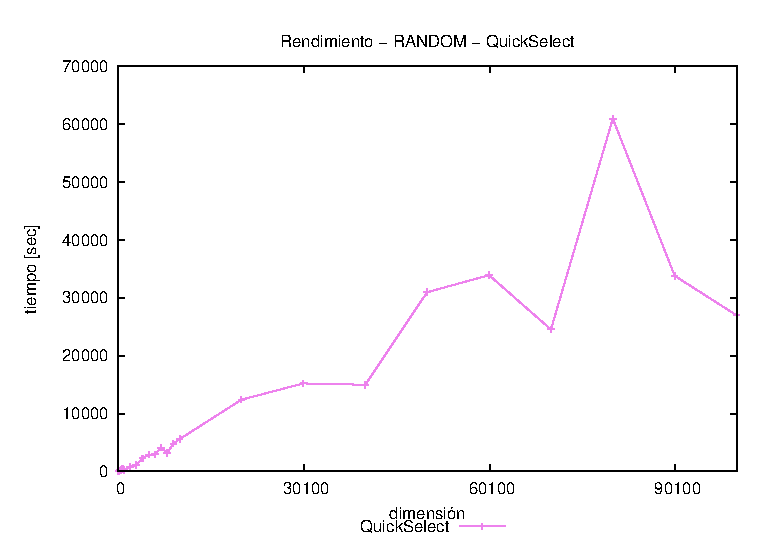
\includegraphics[width=5cm,height=3.5cm]{randomqs2}\\
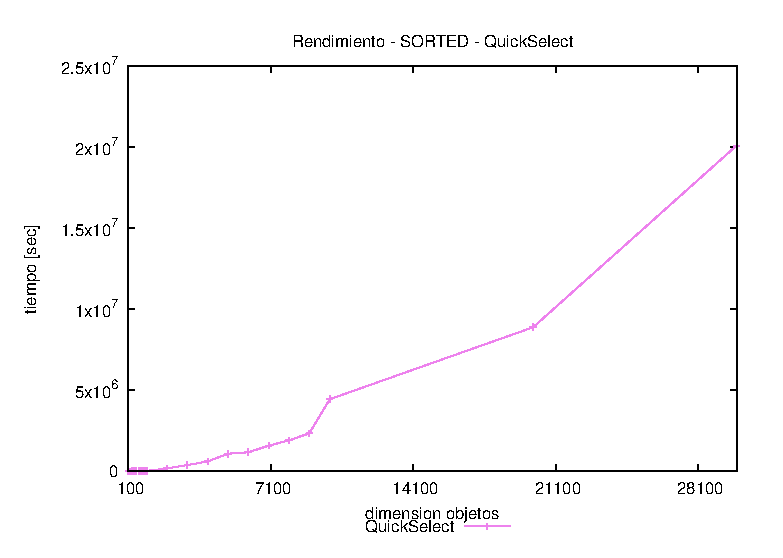
\includegraphics[width=5cm,height=4cm]{sortedqs2}
\column{.5\textwidth}
\centering
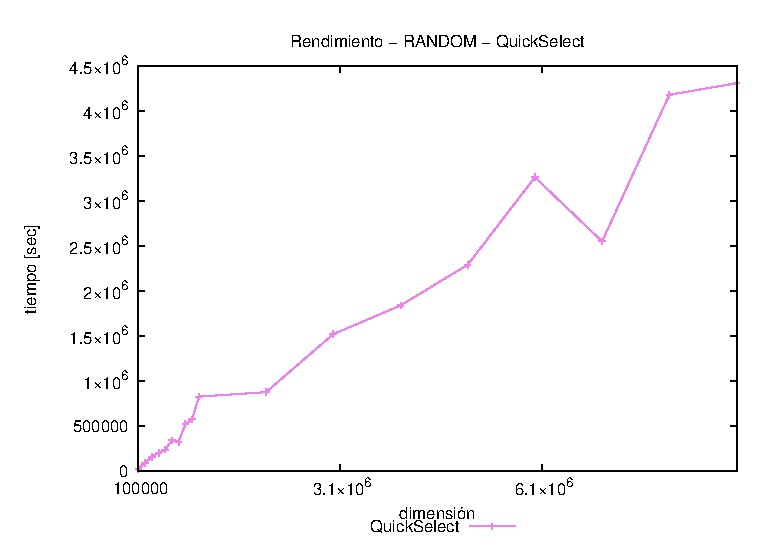
\includegraphics[width=5cm,height=4cm]{randomqs1}\\
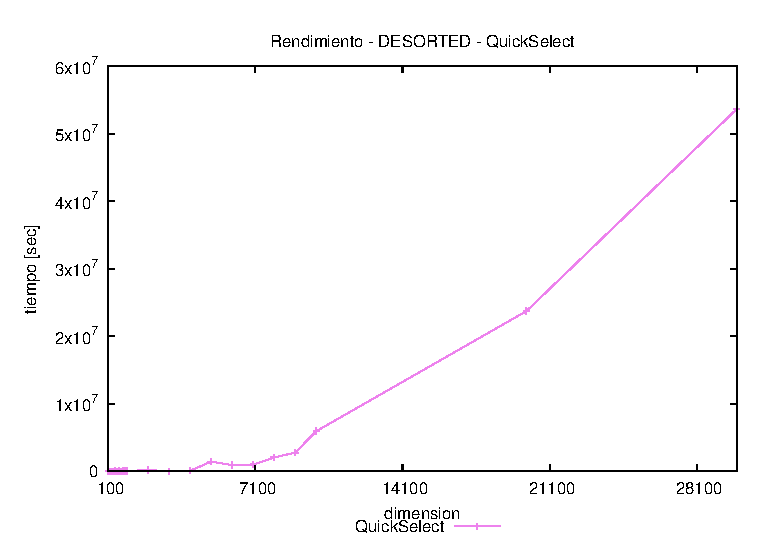
\includegraphics[width=5cm,height=4cm]{desortedqs2}
\end{columns}
\end{frame}

%%%%%%%%%%%%%%%%%%%% BFPRT    %%%%%%%%%%%%%%%%%%
\subsection{Mediana de medianas no iterada}


\begin{frame}
  BFPRT (Mediana de medianas no iterada)
  \begin{itemize}
  	\item Precisi�n: $98\sim100\%$ en todos los casos.
  	\item Reduce el conjunto muestral a $\frac{n}{5}$ para obtener una mediana aproximada en ($O(n\ lg(n)))$.
  	\item Dependiendo del algoritmo de ordenamiento subyacente BFPRT puede variar al peor caso ($O(n^2)$).
  \end{itemize}
\end{frame}

\begin{frame}
\begin{columns}[t]
\column{.5\textwidth}
\centering
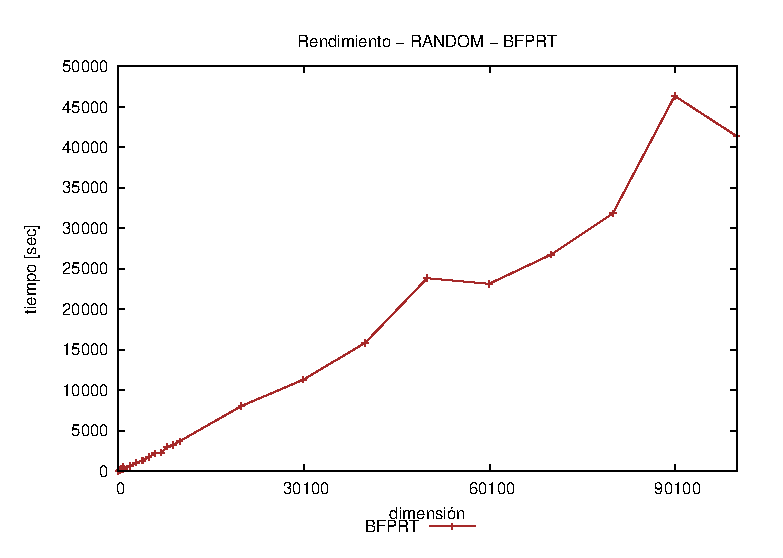
\includegraphics[width=5cm,height=4cm]{randombfprt2}\\
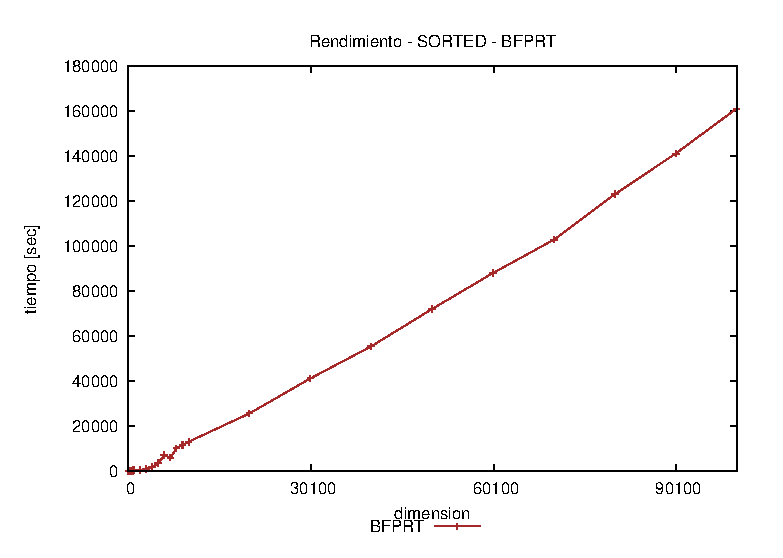
\includegraphics[width=5cm,height=4cm]{sortedbfprt2}
\column{.5\textwidth}
\centering
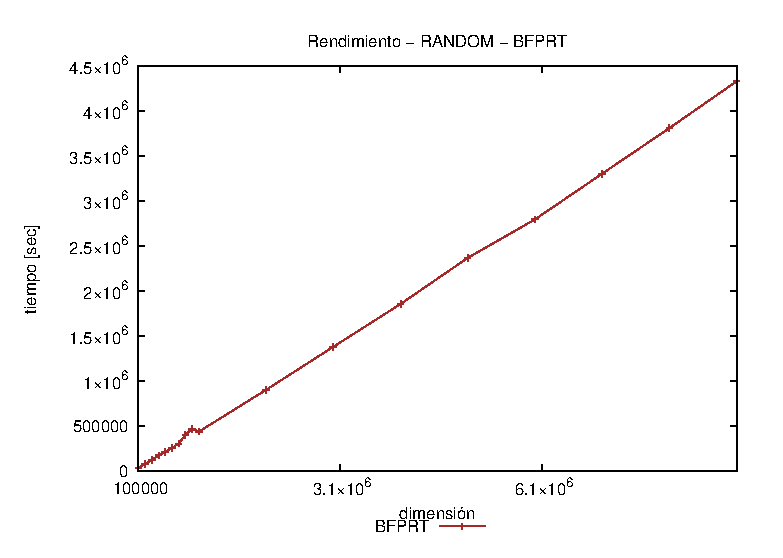
\includegraphics[width=5cm,height=4cm]{randombfprt1}\\
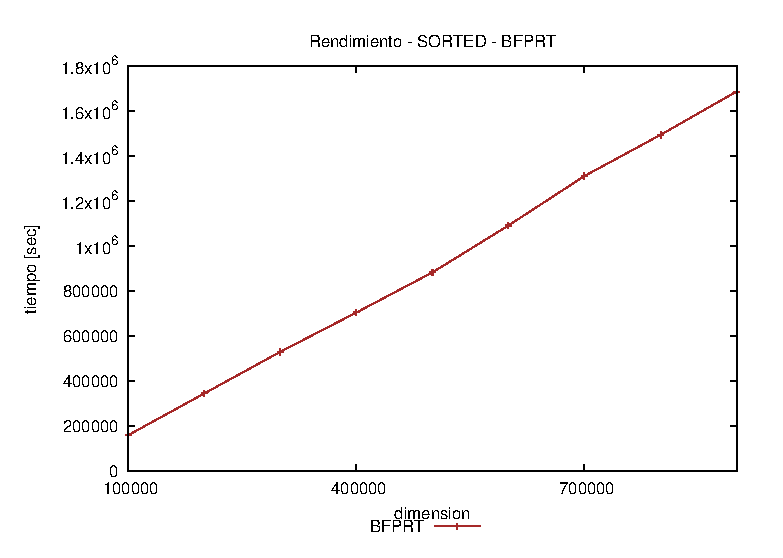
\includegraphics[width=5cm,height=4cm]{sortedbfprt1}
\end{columns}
\end{frame}


\begin{frame}
\begin{columns}[t]
\column{.5\textwidth}
\centering
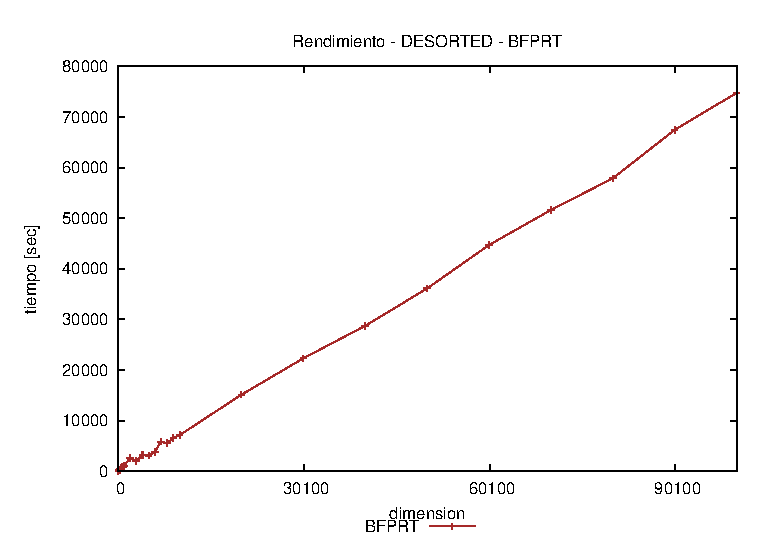
\includegraphics[width=5cm,height=3.5cm]{desortedbfprt2}
\column{.5\textwidth}
\centering
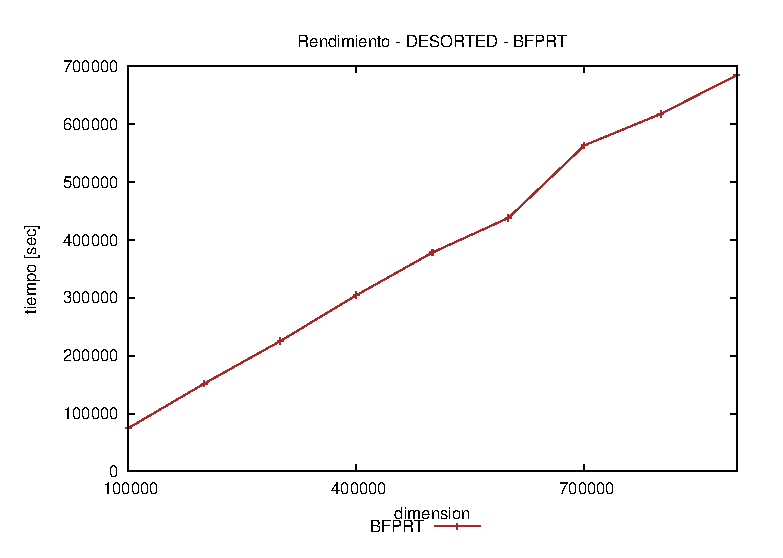
\includegraphics[width=5cm,height=4cm]{desortedbfprt1}
\end{columns}
\end{frame}

%%%%%%%%%%%%%%%%%%%% iBFPRT    %%%%%%%%%%%%%%%%%%

\subsection{Mediana de medianas iterada versus versi�n no iterada}



\begin{frame}
  iBFPRT (Mediana de medianas iterada)
  \begin{itemize}
  	\item Precisi�n:  $94\%$ a $99\%$ para el caso promedio y entre $84\%$ a $99\%$ para el peor caso.
  	\item Iterativamente reduce el conjunto muestral en $\frac{n}{5}$ y luego los divide en $\frac{n}{k}$ conjuntos extrayendo la mediana de un conjunto de tama�o $k$ fijo.
  	\item Provee de una mediana aproximada en tiempo ($O(n)$) en peor caso.
  \end{itemize}
\end{frame}

\begin{frame}
\begin{columns}[t]
\column{.5\textwidth}
\centering
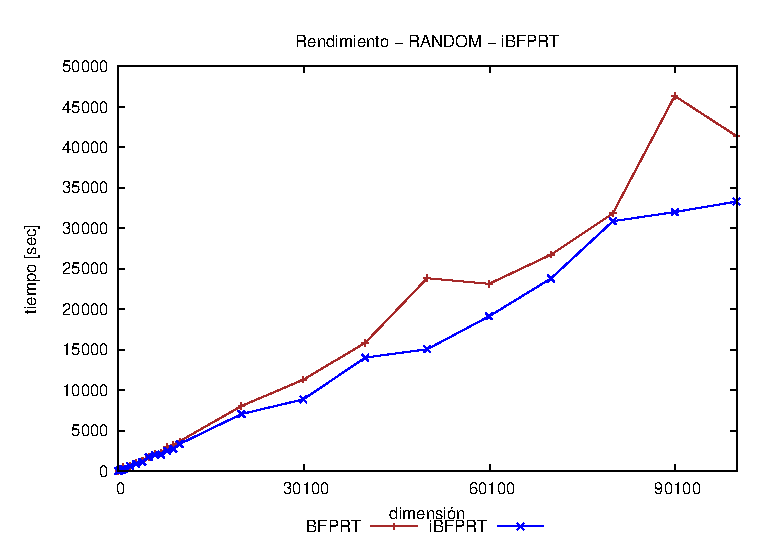
\includegraphics[width=5cm,height=4cm]{randomibfprt2}\\
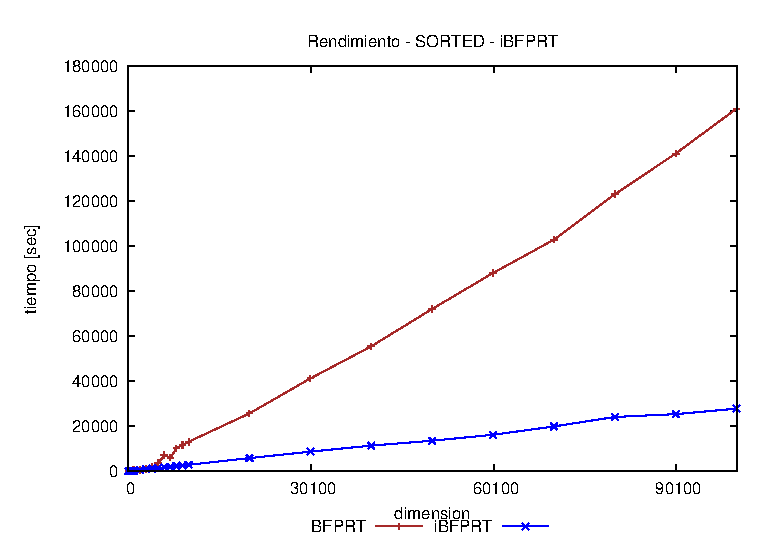
\includegraphics[width=5cm,height=4cm]{sortedibfprt2}
\column{.5\textwidth}
\centering
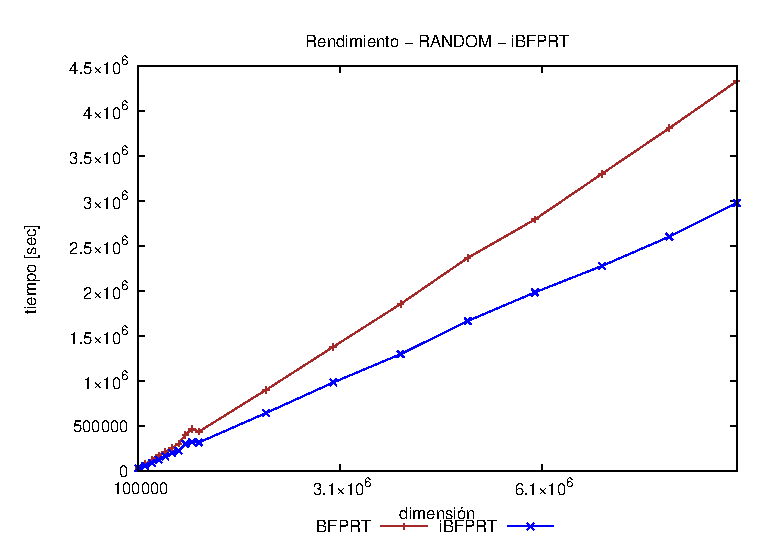
\includegraphics[width=5cm,height=4cm]{randomibfprt1}\\
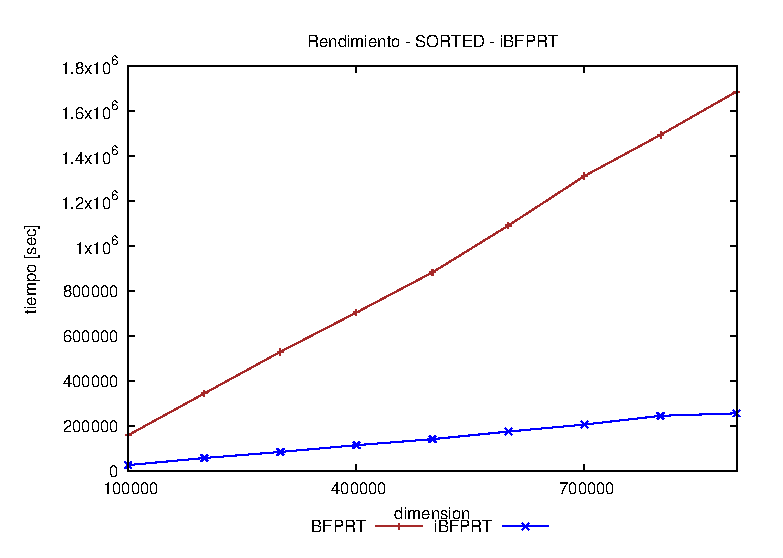
\includegraphics[width=5cm,height=4cm]{sortedibfprt1}
\end{columns}
\end{frame}


\begin{frame}
\begin{columns}[t]
\column{.5\textwidth}
\centering
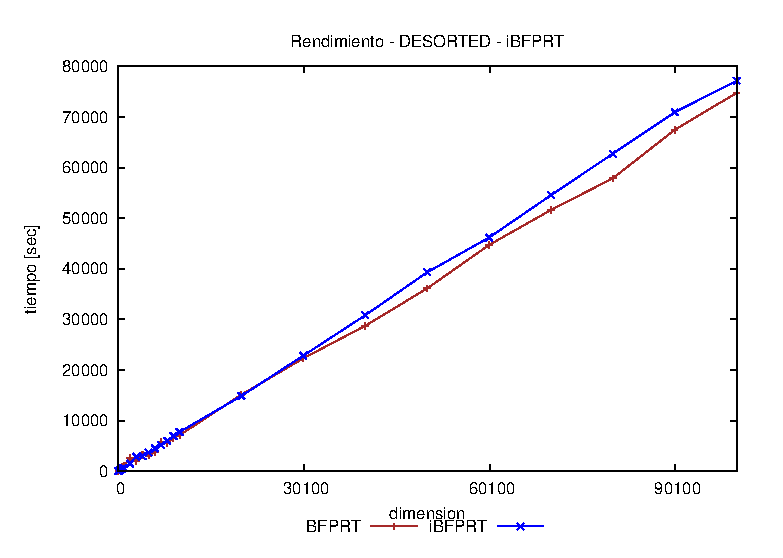
\includegraphics[width=5cm,height=3.5cm]{desortedibfprt2}
\column{.5\textwidth}
\centering
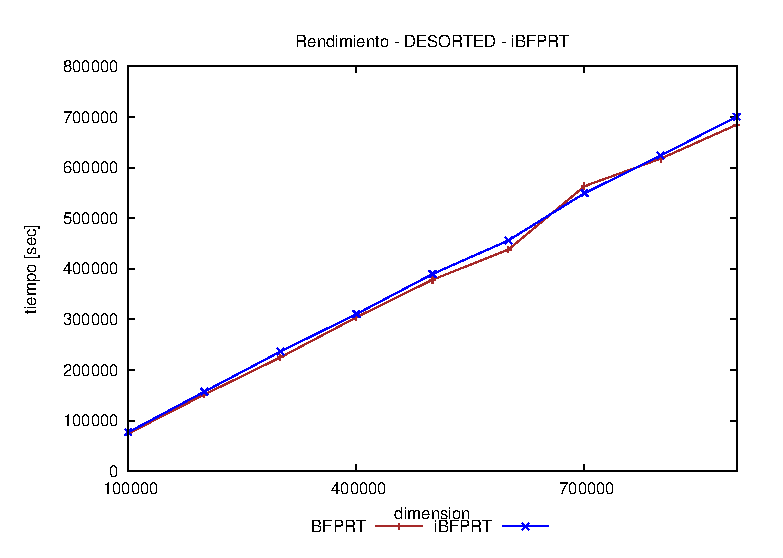
\includegraphics[width=5cm,height=4cm]{desortedibfprt1}
\end{columns}
\end{frame}


%%%%%%%%%%%%%%%%%%%%% IQM    %%%%%%%%%%%%%%%%%%
\subsection{Selecci�n introspectiva de mediana aproximada}



\begin{frame}
  IntrospectiveQuickMedian
\end{frame}
\begin{frame}
\centering
		
\includegraphics[height=\textheight]{wat}
\end{frame}

\begin{frame}
\centering
\scalebox{.6}{\parbox{\linewidth}{%
    \begin{algorithm}[H]
    \begin{algorithmic}[1]
    \REQUIRE $J$ arreglo de datos desordenados, $k$ el largo de la lista temporal $K$, $i,j$ son los l�mites del arreglo $J$
    \ENSURE $A_{\frac{|A|}{2}}$ es la mediana aproximada de $J$
    \IF{recursi�n en peor caso}
    	\STATE $A \leftarrow []$
    	\STATE $i \leftarrow 0$
    	\WHILE{$i+k<|A|$}
    		\STATE $K \leftarrow A_{i...min(i+k,|A|)}$
    		\STATE $K \leftarrow ordenar(K)$
    		\STATE $insertar K_{\frac{|K|}{2} en A}$
    		\STATE $i \leftarrow i+k$
    	\ENDWHILE
    	\STATE $A \leftarrow ordenar(A)$
    	\RETURN $medianaDeMedianas(A)$
    \ELSE
    	\IF{$p \neq \frac{|A|}{2}$}
    		\STATE $p \leftarrow obtenerPivote(A, i, j)$
    		\STATE $p \leftarrow particionar(A, i, j)$
    		\IF{$p > \frac{|A|}{2}$}
    			\STATE $i \leftarrow p$
    		\ELSE
    			\STATE $j \leftarrow p$
    		\ENDIF
    		\RETURN $IntrospectiveQuickMedian(A,i,j)$
    	\ELSE
    		\RETURN $p$
    	\ENDIF
    \ENDIF
    
    \end{algorithmic}
    \caption{Selecci�n de mediana aproximada utilizando introspecci�n}
    \end{algorithm}
}}
\end{frame}



\begin{frame}
  IntrospectiveQuickMedian (Mediana de medianas iterada)
  \begin{itemize}
  	\item Precisi�n:  $99\%$ a $100\%$ para el caso promedio y  $85\%$ a $99\%$ en el peor caso.
  	\item Versi�n h�brida entre QuickSelect y iBFPRT.
  	\item Provee de una mediana aproximada en tiempo ($O(n)$) en peor caso.
	\item Mejora la precisi�n del caso promedio de iBFPRT.
  \end{itemize}
\end{frame}

\begin{frame}
\begin{columns}[t]
\column{.5\textwidth}
\centering
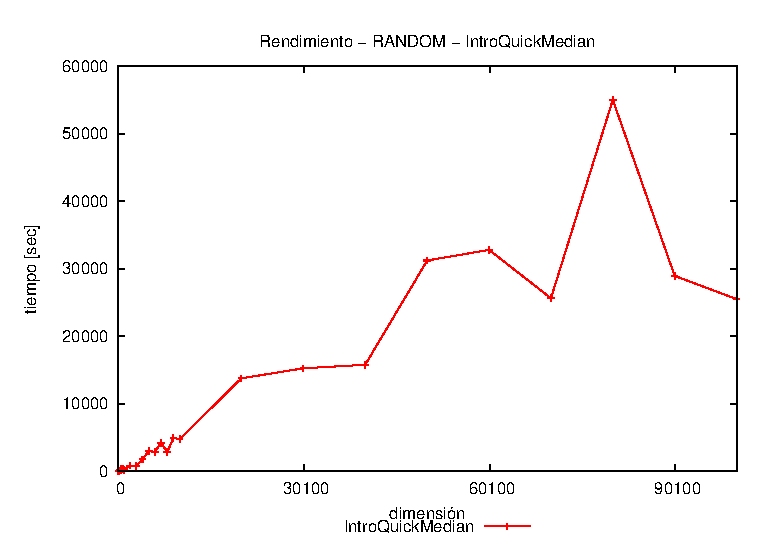
\includegraphics[width=5cm,height=4cm]{randomiqm2}\\
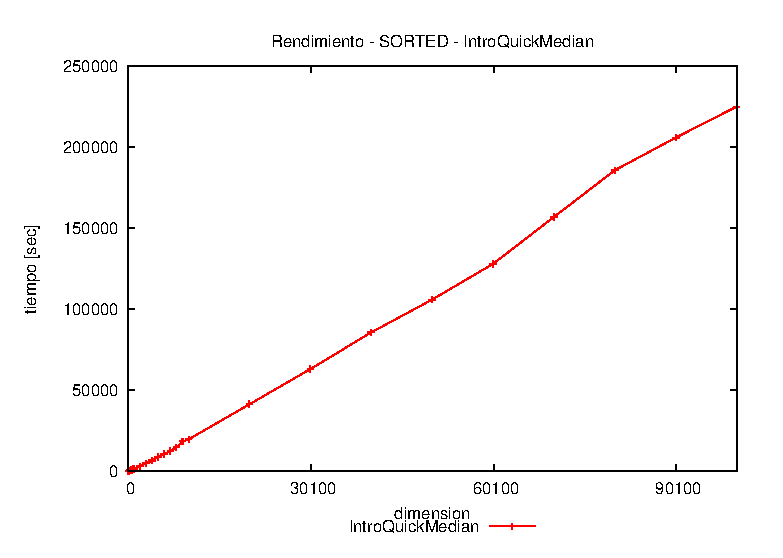
\includegraphics[width=5cm,height=4cm]{sortediqm2}
\column{.5\textwidth}
\centering
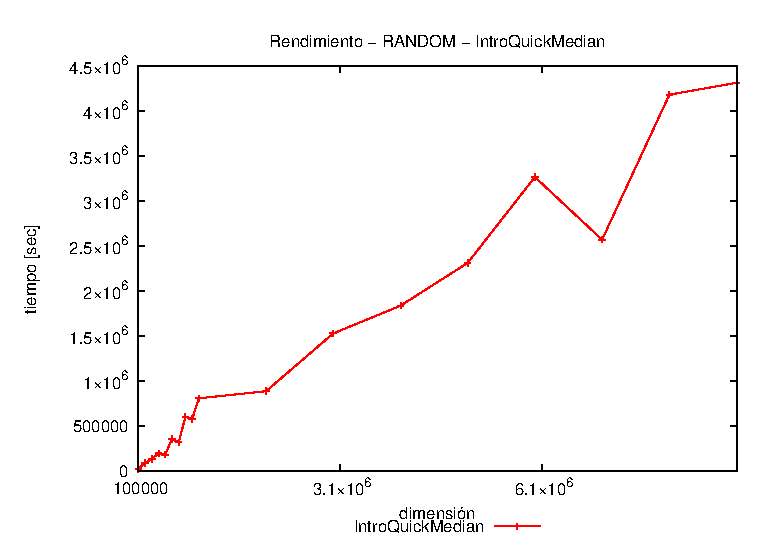
\includegraphics[width=5cm,height=4cm]{randomiqm1}\\
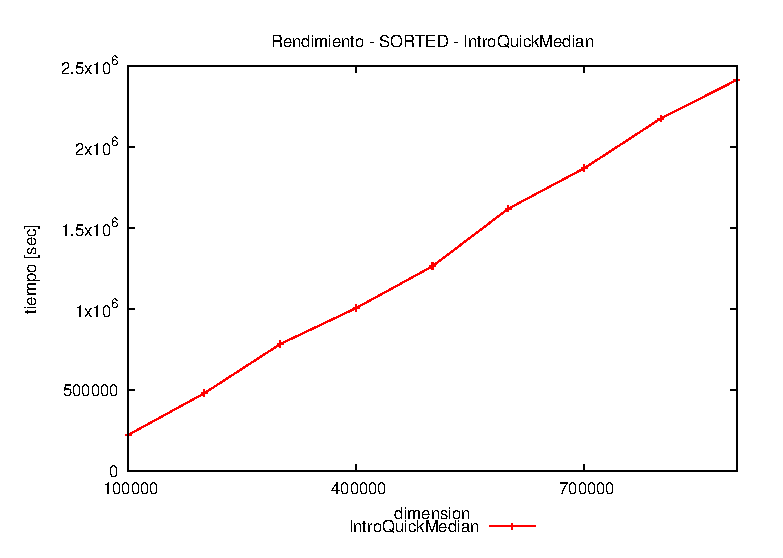
\includegraphics[width=5cm,height=4cm]{sortediqm1}
\end{columns}
\end{frame}


\begin{frame}
\begin{columns}[t]
\column{.5\textwidth}
\centering
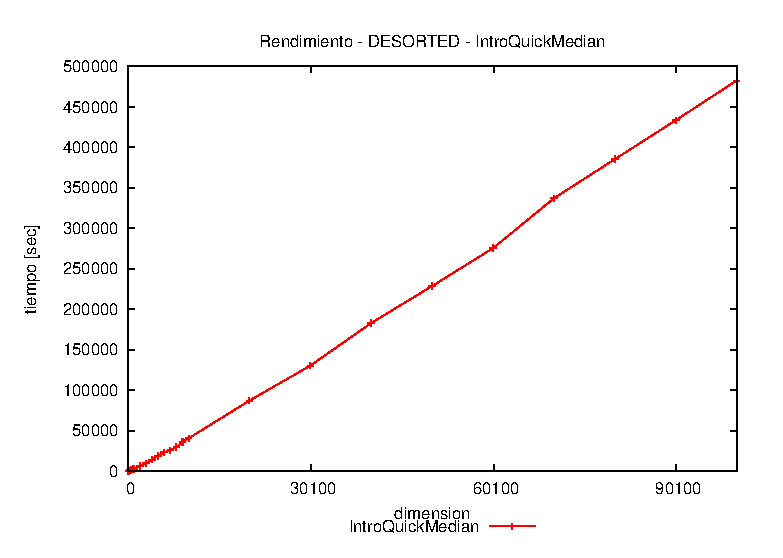
\includegraphics[width=5cm,height=3.5cm]{desortediqm2}
\column{.5\textwidth}
\centering
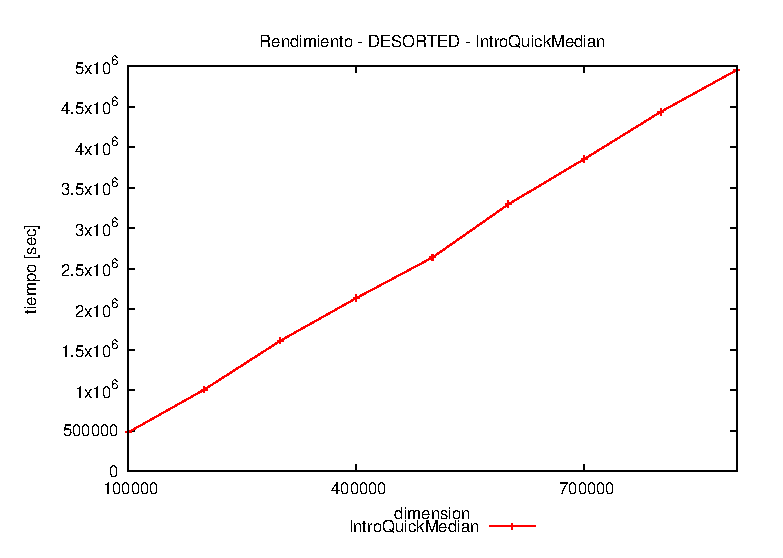
\includegraphics[width=5cm,height=4cm]{desortediqm1}
\end{columns}
\end{frame}

%%%%%%%%%%%%%%%%%%%% RESUMEN    %%%%%%%%%%%%%%%%%%
\section{Resumen y comparaci�n final}


\begin{frame}
  Resumen de los experimentos - Tiempo de ejecuci�n
  \begin{itemize}
  	\item BFPRT es el algoritmo m�s estable entre todos.
  	\item iBFPRT es el algoritmo m�s rapido de todos. 
  	\item Los algoritmos basados en QuickSelect e iBFPRT son erraticos en el caso promedio.
	\item Todos los algoritmos describen un comportamiento uniforme para el peor caso.
  \end{itemize}
\end{frame}

\begin{frame}
\begin{columns}[t]
\column{.5\textwidth}
\centering
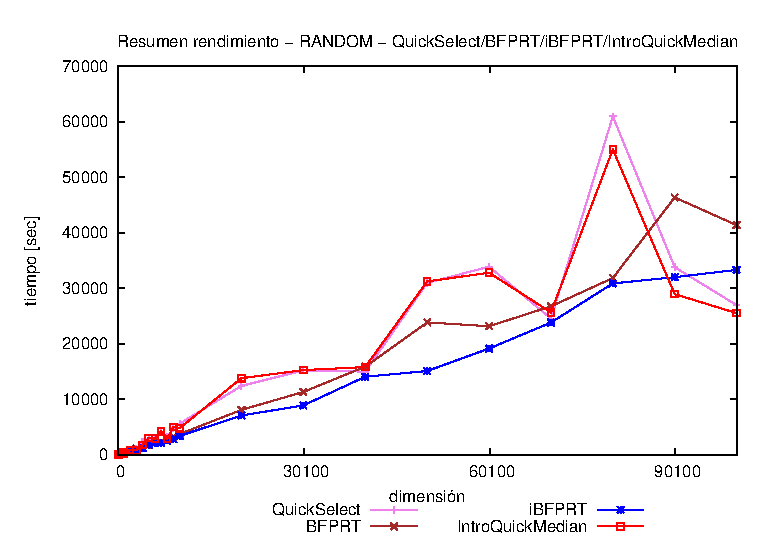
\includegraphics[width=5cm,height=4cm]{randomsummary2}\\
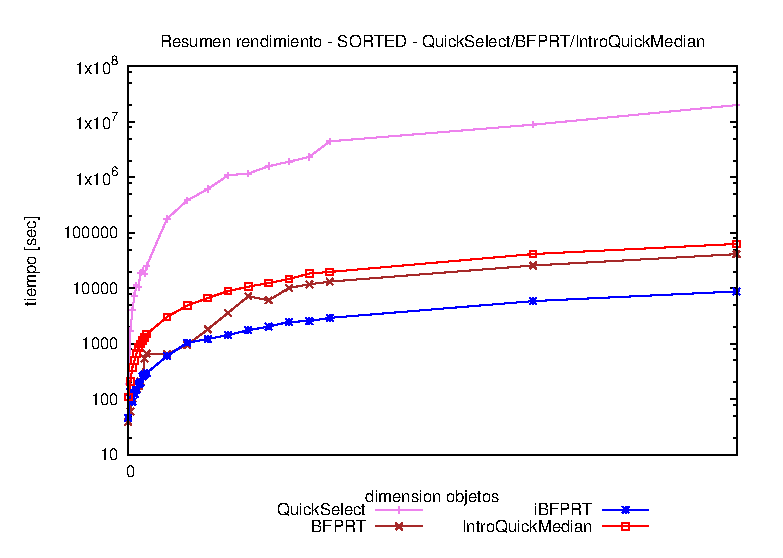
\includegraphics[width=5cm,height=4cm]{sortedsummary2}
\column{.5\textwidth}
\centering
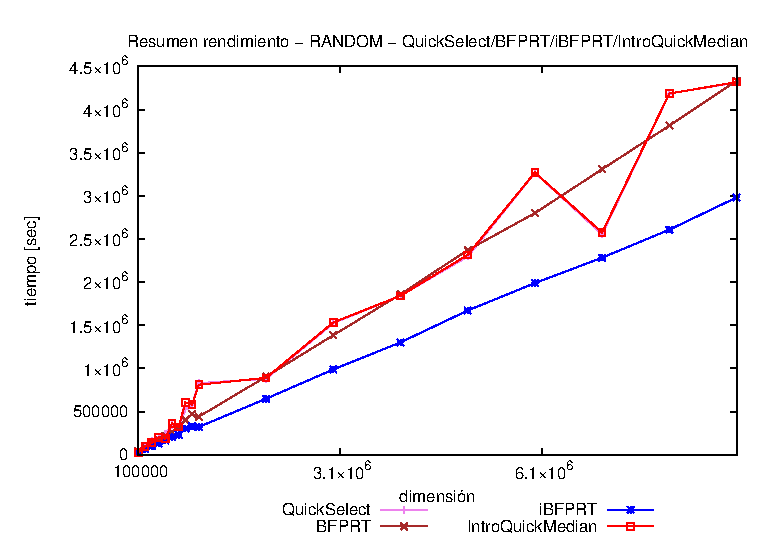
\includegraphics[width=5cm,height=4cm]{randomsummary1}\\
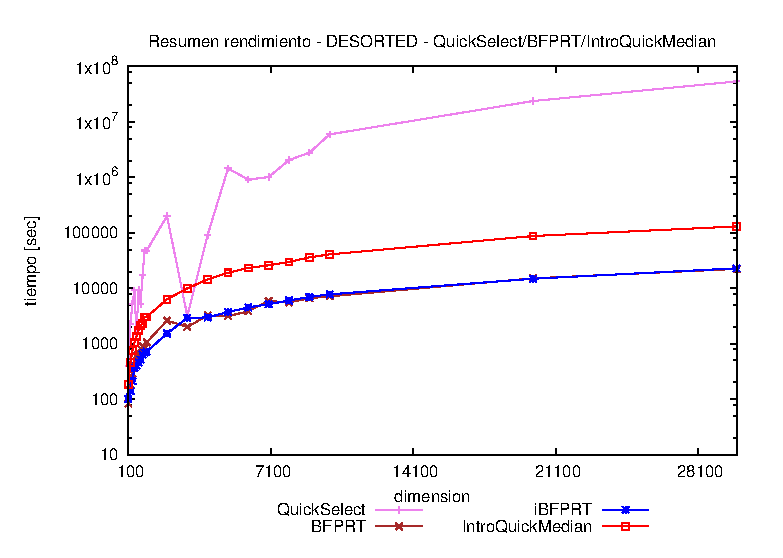
\includegraphics[width=5cm,height=4cm]{desortedsummary2}
\end{columns}
\end{frame}


\begin{frame}
  Resumen de los experimentos - Precisi�n
  \begin{itemize}
  	\item IntrospectiveQuickMedian presenta la mayor precisi�n en el caso promedio, junto con QuickSelect.
  	\item IntrospectiveQuickMedian en la mayor�a de los casos describe un comportamiento similar a iBFPRT.
	\item A medida que aumenta el tama�o del conjunto de datos, todos los algoritmos comienzan incrementar su precisi�n para el caso promedio.
  \end{itemize}
\end{frame}


\begin{frame}
\begin{columns}[t]
\column{.5\textwidth}
\centering
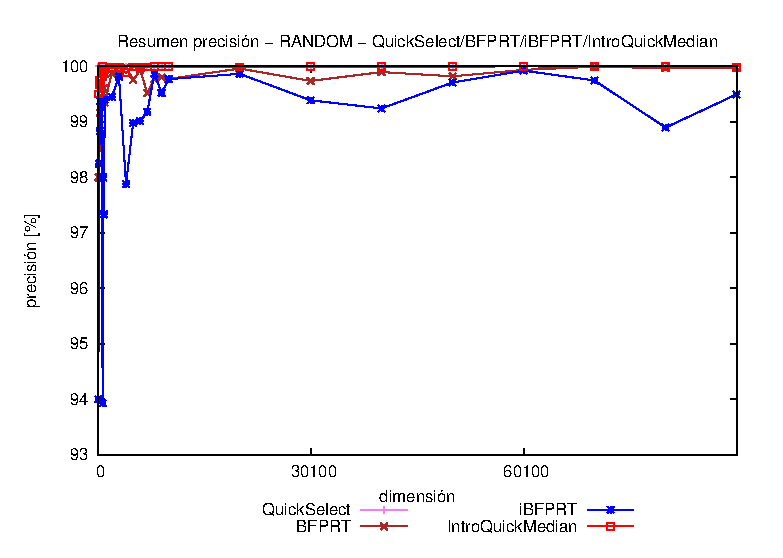
\includegraphics[width=5cm,height=4cm]{randomprecision1}\\
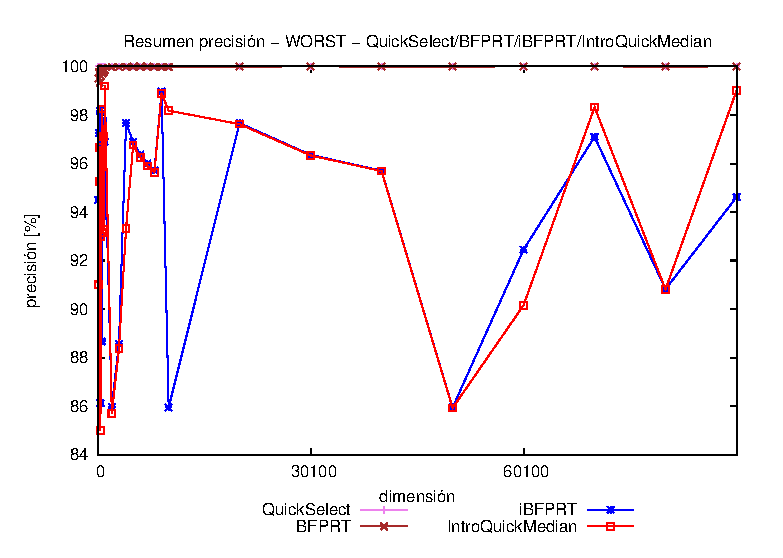
\includegraphics[width=5cm,height=4cm]{desortedprecision1}
\column{.5\textwidth}
\centering
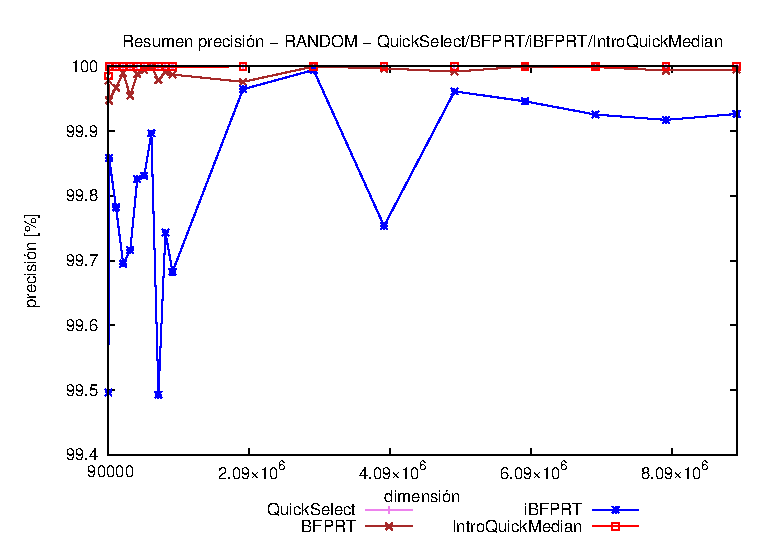
\includegraphics[width=5cm,height=4cm]{randomprecision2}\\
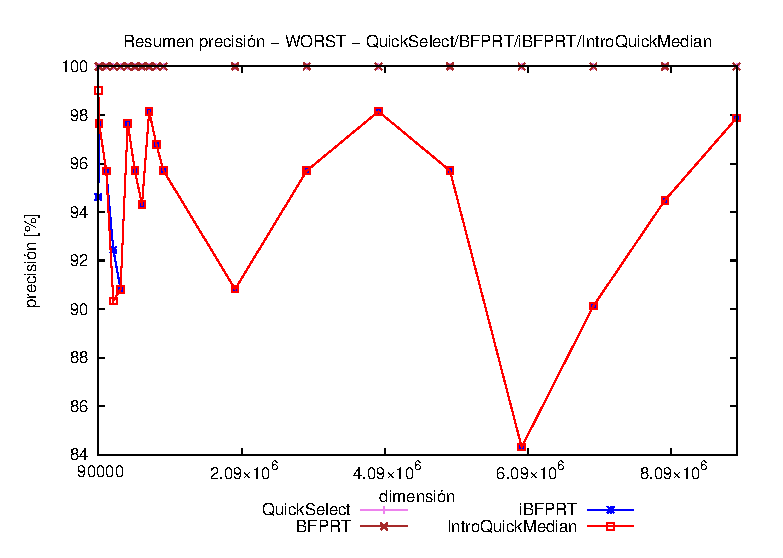
\includegraphics[width=5cm,height=4cm]{desortedprecision2}
\end{columns}
\end{frame}



\section{Trabajo Futuro}

\begin{frame}
  Trabajo futuro
	\begin{itemize}
		\item Investigar el efecto que produce reducir el espacio muestral utilizando la t�cnica empleada en BFPRT no iterado sobre IntrospectiveQuickMedian
		\item Investigar el efecto que tiene este algoritmo de selecci�n de medianas en algoritmos de selecci�n basados en pivotes.
		\item Investigar el efecto que tiene el criterio de selecci�n de espacio muestral sobre la condici�n de introspecci�n.
	\end{itemize}
\end{frame}


\begin{frame}
\centering
		FIN
\end{frame}



\end{document}
